\documentclass{../res/univ-projet}

%Import des packages utilisés pour le document
\usepackage[utf8x]{inputenc}
\usepackage[francais]{babel}
\usepackage[T1]{fontenc}
%\usepackage{array}
%\usepackage{hyperref}
%\usepackage{tabularx, longtable}
%\usepackage[table]{xcolor}
%\usepackage{fancyhdr}
%\usepackage{lastpage}

\definecolor{gris}{rgb}{0.95, 0.95, 0.95}

%Redéfinition des marges
%\addtolength{\hoffset}{-2cm}
%\addtolength{\textwidth}{4cm}
\addtolength{\topmargin}{-1cm}
\addtolength{\textheight}{1cm}
\addtolength{\headsep}{0.8cm} 
\addtolength{\footskip}{-0.2cm}


%Import page de garde et structures pour la gestion de projet
%\usepackage{structures}

%Variables
\logo{../res/logo_univ.png}
\title{Cahier des Recettes}
\author{Pierre \bsc{Balmelle}, Lucas \bsc{Barbay}}
\projet{Projet PGP}
\projdesc{Etude et implantation d'un outil graphique de gestion de clé PGP}
\filiere{Master 1 SSI }
\matiere{Conduite de projet}
\version{0.5}
\relecteur{Olivier \bsc{Thibault}}
\signataire{}
\date{\today}


\histentry{0.5}{15/12/2014}{Respect de la STB v0.4 et ajout des données de test.}
\histentry{0.4}{05/12/2014}{Ajout de toutes les procédures liées aux commandes GPG.}
\histentry{0.3}{24/11/2014}{Respect de la STB v0.3.}
\histentry{0.2}{15/11/2014}{Ajout des parties Introduction, Documents applicables et de référence, Environnement de test, Responsabilités,
Stratégie de tests, Gestion des anomalies.}
\histentry{0.1}{31/10/2014}{Version initiale.}


% -- Début du document -- %
\begin{document}

%Page de garde
\maketitle
\newpage
%La table des matières
\tableofcontents
\newpage

\section{Introduction}

% Présentation succinte du sujet et hyp de travail.
Ce document est le Cahier de Recette (CDR) de la réalisation d'une interface graphique pour le logiciel GnuPG.
Cette interface permettra d'utiliser complètement l'outil OpenPGP de façon intuitive et pédagogique de façon 
à être accessible même par des personnes ayant des connaissances limitées dans le domaine de l'informatique. 

\subsection{Fonctionnalités du logiciel}
Le logiciel est une interface graphique pour le GnuPG (implémentation GNU du standart OpenPGP).
Les différents cas d'utilisations :
\begin{itemize}
 \item Exécuter une action GPG.
 \item Chiffrement/déchiffrement, signature/vérification.
 \item Affichage des commandes et des erreurs.
 \item Choix du fichier de configuration.
 \item Modifications de la toile de confiance.
 \item Attaque sur la seconde pré-image.
\end{itemize}

\subsection{Liste des objets à tester}
Nous avons dégagé 3 objets à tester : 
\begin{itemize}
 \item L'interface graphique des fonctions GnuPG.
 \item La visualisation de la toile de confiance.
 \item L'implémentation de l'attaque sur les secondes pré-images. 
\end{itemize}

L'interface graphique permettra d'utiliser chaque commande et option de GPG et ce de façon le plus intuitif possible. Nous
devrons tester le résultat des commandes ainsi que le temps d'exécution pour satisfaire le client en terme de fluidité de l'interface.

La toile de confiance réprésentera un schéma des différentes personnes d'un réseau qui seront liées par des clés.
Les clés seront de couleurs différentes en fonction de la confiance accordée à chacun.

Enfin, il nous faudra tester l'implémentation de l'attaque. 


\section{Documents applicables et de référence}
% Liste des
% - Références des documents quidefinissent formellement les principes
%   directeurs et le hypothèse de travail prise en compte pour l'établissement de la spécification.
% - Références des documents cités dans la STB au titre d'explication ou de justification.
Différents documents de référence :
\begin{itemize}
\item Définitions du standard OpenPGP \href{file:../../ressources/openPGP/rfc4880-en.pdf}{RFC 4880}
  et \href{file:../../ressources/openPGP/rfc2440-fr.pdf}{RFC 2440}.
\item Le logiciel \href{https://www.gnupg.org/}{GnuPG} (GNU Privacy Guard) implantation Open Source
  de OpenPGP.
\item La \href{https://www.gnupg.org/gph/fr/manual.html#AEN541}{toile de confiance} de GnuPG.
\item Editeurs graphiques existant
  (\href{http://www.gnupg.org/related_software/frontends.en.html}{KGpg, GPA, Seahorse}).
\item Exemple de visualisation d'une toile de confiance sur le site de 
  \href{https://www.archlinux.org/master-keys/#visualization}{archlinux}.
\end{itemize}

\section{Terminologie et sigles utilisés}
\textcolor{blue}{
  Le glossaire est dans un fichier à part, il est commun aux autres documents de gestion de projet.
}

\section{Environnement de test}
\subsection{Sites de réalisation des tests}
Les test seront réalisés soit sur le site de l'université soit au domicile des deux testeurs sur leur machine personnelle.



\subsection{Configurations matérielles utilisées}
Voici la configuration des machines personnelles des deux testeurs :
\begin{itemize}
 \item PC n°1 : Un ordinateur portable équipé de Kali Linux 1.0(Debian) 64 bits sous Gnome avec un processeur Intel i5-3210M @ 2.50GHz et 6Go de RAM.
 \item PC n°2 : Un ordinateur portable équipé de Xubuntu 64 bits avec un processeur Intel i7-2630QM.
 @ 2.00 GHz et 6Go de RAM.
\end{itemize}
Seront également utilisées des machines virtuelles pour répondre aux besoins du client sur la compatibilité de l'interface (KDE et GNOME obligatoire,
WINDOWS optionnel).

\subsection{Outils de tests mis en oeuvre}
Le module Qt Test de Qt.
Les modules CxxTest et CppUnit pourront être utilisés.

\subsection{Jeux de données/Bases de données}
Nous aurons comme jeu de données les différentes clés contenues dans le trousseau de test.


\subsection{Contraintes à prendre en compte}
Chaque procédure de test devra être réalisée :
\begin{itemize}
 \item Sous KDE.
 \item Sous GNOME.
 \item Avec deux interfaces graphiques ouvertes avec des profils différents.
\end{itemize}
Chaque procédure de test sera si possible réalisée à l'aide de l'api Qt (automatiquement), et à l'aide de l'interface (manuellement).



\section{Responsabilités}

  La création et la gestion des procédures de test sera effectuée par les responsables qualité de l'équipe. Chaque équipe travaillant au développement d'un composant est chargée de tester celui-ci continuellement et de publier les résultats des tests.
  
  Afin d'assurer la compréhension générale du code source, toute l'équipe peut et est encouragée à signaler une anomalie détectée au cours du développement : soit elle est résolue par la même personne/groupe, soit cette personne/ce groupe transmet les résultats 
  des tests à une autre personne/groupe afin que celle-ci travaille à la réparation de l'anomalie.
  
  À tout moment une équipe peut reporter des anomalies dans une procédure de test. Dans ce cas, les responsables techniques concernés travailleront à améliorer la procédure incriminée et diffuseront les mises à jour à l'ensemble de l'équipe.

  Dans tous les cas, les instructions incluses dans la partie \emph{Gestion des anomalies} sont à respecter.


\section{Stratégies de tests}

\subsection{Description de l'approche et des phases de test}
Dès qu'un test pour un composant sera réalisable, il sera fait. Ces tests devront être appliqués à chaque nouvelle version du composant.


\subsection{Campagne de test}

Les différentes campagnes de tests correspondront aux livrables envoyés au client.

\subsection{Ordre d'exécution des tests}

L'ordre d'exécution des tests suivra l'ordre du plan de développement.

\subsection{Critères d'arrêt des tests}

Un test est considéré comme échoué dès qu'une de ses étapes échoue, produit un résultat non attendu ou est impossible à mener à bout.


\section{Gestion des anomalies}

Quand des anomalies seront détectées, la procédure suivante devra être respectée:
  \begin{itemize}
   \item Création d'un mémo précisant l'anomalie rencontrée ainsi que les conditions de reproduction de l'anomalie si disponibles et l'état du système lors de l'apparition de l'anomalie.  
   Un identifiant unique lui sera attribué.
   \item Ajout d'une entrée au journal de test précisant la date du test, la référence du mémo, le nom ainsi que la référence de l'exigence de 
   qualité non respectée.
   \item Diffusion de la note à l'équipe de développement.
   \item Une personne est désignée pour corriger l'anomalie.
   \item Cette personne vérifie la gravité de l'anomalie, puis la corrige.
   \item Une deuxième personne s'assure que l'anomalie est bien corrigée.
   \item Une fois la vérification effectuée, la personne ayant corrigé l'anomalie établit un contre-mémo portant le même identifiant et précisant les raisons supposées 
   de l'anomalie ainsi que les corrections mises en place.
  \end{itemize}
  

  Dans la pratique, la gestions des anomalies sera faite à l'aide de l'outil \emph{issue tracker} de
  la plate-forme d'hébergement Gitlab. Cet outil permet la création de files de discussion associées à un bug
  de l'application. Il laisse aussi la possibilité aux collaborateurs du projet de prendre en charge 
  une \emph{issue} particulière. L'ensemble des \emph{issues} ouvertes est conservé par Gitlab ainsi
  que les files de discussion associés permettant de parcourir l'historique des bugs du projet.


\section{Procédures de test}

\begin{center}
    %---------------------------------------Test N° 1------------------------------------------------------------------------------
    \begin{tabular}{|c|p{5cm}|p{5cm}|p{1.5cm}|p{1.5cm}|}
      \hline
      \multicolumn{3}{|l|}{Objet testé : Interface Graphique} & \multicolumn{2}{c|}{Version : 0.1}\\ \hline
      \multicolumn{5}{|l|}{Objectif de test : Création de clé}\\ \hline
      \multicolumn{3}{|l|}{Procédure n° 1} & \multicolumn{2}{p{3cm}|}{Pré-requis : }\\ \hline
      \multicolumn{1}{|c|}{N°} & \multicolumn{1}{c|}{Actions} & \multicolumn{1}{c|}{Résultats attendus} & 
      \multicolumn{1}{c|}{Exigence} & \multicolumn{1}{c|}{OK/KO}\\ \hline
      1 & Créer une clé & commande lancée : \texttt{"gpg -\-gen-key"} &  & \\
      2 &  &  &  & \\
      3 &  &  &  & \\ 
      4 &  &  &  & \\
      5 &  &  &  & \\
      6 &  &  &  & \\
      7 &  &  &  & \\
      8 &  &  &  & \\
      9 &  &  &  & \\
      10 &  &  &  &\\ 
	\hline
    \end{tabular}
    \vskip 2.2cm



 %---------------------------------------Test N° 2------------------------------------------------------------------------------
    \begin{tabular}{|c|p{5cm}|p{5cm}|p{1.5cm}|p{1.5cm}|}
      \hline
      \multicolumn{3}{|l|}{Objet testé : Toile de confiance} & \multicolumn{2}{c|}{Version : 0.1}\\ \hline
      \multicolumn{5}{|l|}{Objectif de test : Tout changement de confiance est répercuté sur la toile de confiance.}\\ \hline
      \multicolumn{3}{|l|}{Procédure n° 2} & \multicolumn{2}{p{3cm}|}{Pré-requis : }\\ \hline
      \multicolumn{1}{|c|}{N°} & \multicolumn{1}{c|}{Actions} & \multicolumn{1}{c|}{Résultats attendus} & 
      \multicolumn{1}{c|}{Exigence} & \multicolumn{1}{c|}{OK/KO}\\ \hline
      1 & Changer la confiance d'une clé & La représentation de cette clé a changé de couleur en fonction de la nouvelle confiance &  & \\
      2 &  &  &  & \\
      3 &  &  &  & \\ 
	  4 &  &  &  & \\
      5 &  &  &  & \\
	  6 &  &  &  & \\
      7 &  &  &  & \\
      8 &  &  &  & \\
      9 &  &  &  & \\
      10 &  &  &  &\\ 
	\hline
    \end{tabular}
    \vskip 2.2cm



 %---------------------------------------Test N° 3------------------------------------------------------------------------------
    \begin{tabular}{|c|p{5cm}|p{5cm}|p{1.5cm}|p{1.5cm}|}
      \hline
      \multicolumn{3}{|l|}{Objet testé : Attaque seconde pré-image} & \multicolumn{2}{c|}{Version : 0.1}\\ \hline
      \multicolumn{5}{|l|}{Objectif de test : La clé produite a la même seconde pré-image que celle donnée.}\\ \hline
      \multicolumn{3}{|l|}{Procédure n° 3} & \multicolumn{2}{p{3cm}|}{Pré-requis : }\\ \hline
      \multicolumn{1}{|c|}{N°} & \multicolumn{1}{c|}{Actions} & \multicolumn{1}{c|}{Résultats attendus} & 
      \multicolumn{1}{c|}{Exigence} & \multicolumn{1}{c|}{OK/KO}\\ \hline
      1 & Donner une clé publique au programme d'attaque & Le programme renvoie une clé différente avec la même pré-image &  & \\
      2 & Comparer la clé produite avec la clé initiale & Les deux clés ont la même seconde pré-image &  & \\
      3 &  &  &  & \\ 
	  4 &  &  &  & \\
      5 &  &  &  & \\
	  6 &  &  &  & \\
      7 &  &  &  & \\
      8 &  &  &  & \\
      9 &  &  &  & \\
      10 &  &  &  &\\ 
	\hline
    \end{tabular}
    \vskip 2.2cm



 %---------------------------------------Test N° 4------------------------------------------------------------------------------
    \begin{tabular}{|c|p{5cm}|p{5cm}|p{1.5cm}|p{1.5cm}|}
      \hline
      \multicolumn{3}{|l|}{Objet testé : Editeur de texte de l'interface graphique} & \multicolumn{2}{c|}{Version : 0.3}\\ \hline
      \multicolumn{5}{|l|}{Objectif de test : Test de la zone de copier/coller}\\ \hline
      \multicolumn{3}{|l|}{Procédure n° 4} & \multicolumn{2}{p{3cm}|}{Pré-requis : }\\ \hline
      \multicolumn{1}{|c|}{N°} & \multicolumn{1}{c|}{Actions} & \multicolumn{1}{c|}{Résultats attendus} & 
      \multicolumn{1}{c|}{Exigence} & \multicolumn{1}{c|}{OK/KO}\\ \hline
      1 & Coller du texte dans la zone de texte & Le texte s'affiche dans la zone de texte &  & \\
      2 & Cliquer sur "Chiffrer et signer" & La commande exécutée est "gpg -es <texte>" &  & \\
      3 &  &  &  & \\ 
	  4 &  &  &  & \\
      5 &  &  &  & \\
	  6 &  &  &  & \\
      7 &  &  &  & \\
      8 &  &  &  & \\
      9 &  &  &  & \\
      10 &  &  &  &\\ 
	\hline
    \end{tabular}
    \vskip 2.2cm



 %---------------------------------------Test N° 5------------------------------------------------------------------------------
    \begin{tabular}{|c|p{5cm}|p{5cm}|p{1.5cm}|p{1.5cm}|}
      \hline
      \multicolumn{3}{|l|}{Objet testé : Editeur de texte de l'interface graphique} & \multicolumn{2}{c|}{Version : 0.3}\\ \hline
      \multicolumn{5}{|l|}{Objectif de test : Test de la zone de copier/coller}\\ \hline
      \multicolumn{3}{|l|}{Procédure n° 5} & \multicolumn{2}{p{3cm}|}{Pré-requis : }\\ \hline
      \multicolumn{1}{|c|}{N°} & \multicolumn{1}{c|}{Actions} & \multicolumn{1}{c|}{Résultats attendus} & 
      \multicolumn{1}{c|}{Exigence} & \multicolumn{1}{c|}{OK/KO}\\ \hline
      1 & Coller du texte chiffré et signé dans la zone de texte & Le texte s'affiche dans la zone de texte &  & \\
      2 & Cliquer sur "Déchiffrer et vérifier" & La commande exécutée est "gpg -dv <texte>" &  & \\
      3 &  &  &  & \\ 
	  4 &  &  &  & \\
      5 &  &  &  & \\
	  6 &  &  &  & \\
      7 &  &  &  & \\
      8 &  &  &  & \\
      9 &  &  &  & \\
      10 &  &  &  &\\ 
	\hline
    \end{tabular}
    \vskip 2.2cm



 %---------------------------------------Test N° 6------------------------------------------------------------------------------
    \begin{tabular}{|c|p{5cm}|p{5cm}|p{1.5cm}|p{1.5cm}|}
      \hline
      \multicolumn{3}{|l|}{Objet testé : Interface graphique} & \multicolumn{2}{c|}{Version : 0.3}\\ \hline
      \multicolumn{5}{|l|}{Objectif de test : Affichage des commandes et retours gpg}\\ \hline
      \multicolumn{3}{|l|}{Procédure n° 6} & \multicolumn{2}{p{3cm}|}{Pré-requis : }\\ \hline
      \multicolumn{1}{|c|}{N°} & \multicolumn{1}{c|}{Actions} & \multicolumn{1}{c|}{Résultats attendus} & 
      \multicolumn{1}{c|}{Exigence} & \multicolumn{1}{c|}{OK/KO}\\ \hline
      1 & Activer l'affichage des commandes gpg dans l'interface graphique &  &  & \\
      2 & Lancer une commande gpg via l'interface graphique & La commande et les retours sont affichés &  & \\
      3 &  &  &  & \\ 
	  4 &  &  &  & \\
      5 &  &  &  & \\
	  6 &  &  &  & \\
      7 &  &  &  & \\
      8 &  &  &  & \\
      9 &  &  &  & \\
      10 &  &  &  &\\ 
	\hline
    \end{tabular}
    \vskip 2.2cm



 %---------------------------------------Test N° 7------------------------------------------------------------------------------
    \begin{tabular}{|c|p{5cm}|p{5cm}|p{1.5cm}|p{1.5cm}|}
      \hline
      \multicolumn{3}{|l|}{Objet testé : Interface graphique} & \multicolumn{2}{c|}{Version : 0.3}\\ \hline
      \multicolumn{5}{|l|}{Objectif de test : Tester la sélection du profil}\\ \hline
      \multicolumn{3}{|l|}{Procédure n° 7} & \multicolumn{2}{p{3cm}|}{Pré-requis : }\\ \hline
      \multicolumn{1}{|c|}{N°} & \multicolumn{1}{c|}{Actions} & \multicolumn{1}{c|}{Résultats attendus} & 
      \multicolumn{1}{c|}{Exigence} & \multicolumn{1}{c|}{OK/KO}\\ \hline
      1 & Lancer l'interface graphique en ligne de commande avec l'option -P & On peut choisir son profil, et en créer un si besoin &  & \\
      2 & Choisir un profil & L'interface graphique s'affiche &  & \\
      3 & Cliquer sur le bouton "Changer de profil" & On peut choisir son profil, et en créer un si besoin &  & \\ 
	  4 &  &  &  & \\
      5 &  &  &  & \\
	  6 &  &  &  & \\
      7 &  &  &  & \\
      8 &  &  &  & \\
      9 &  &  &  & \\
      10 &  &  &  &\\ 
	\hline
    \end{tabular}
    \vskip 2.2cm



 %---------------------------------------Test N° 8------------------------------------------------------------------------------
    \begin{tabular}{|c|p{5cm}|p{5cm}|p{1.5cm}|p{1.5cm}|}
      \hline
      \multicolumn{3}{|l|}{Objet testé : Toile de confiance} & \multicolumn{2}{c|}{Version : 0.3}\\ \hline
      \multicolumn{5}{|l|}{Objectif de test : Affichage des couleurs de la toile de confiance}\\ \hline
      \multicolumn{3}{|l|}{Procédure n° 8} & \multicolumn{2}{p{3cm}|}{Pré-requis : }\\ \hline
      \multicolumn{1}{|c|}{N°} & \multicolumn{1}{c|}{Actions} & \multicolumn{1}{c|}{Résultats attendus} & 
      \multicolumn{1}{c|}{Exigence} & \multicolumn{1}{c|}{OK/KO}\\ \hline
      1 & Ouvrir la toile de confiance & Toile de confiance affichée &  & \\
      2 & Vérifier que chaque niveau de confiance est représenté par une couleur & Chaque niveau de confiance est représenté par une couleur différente &  & \\
      3 &  &  &  & \\ 
	  4 &  &  &  & \\
      5 &  &  &  & \\
	  6 &  &  &  & \\
      7 &  &  &  & \\
      8 &  &  &  & \\
      9 &  &  &  & \\
      10 &  &  &  &\\ 
	\hline
    \end{tabular}
    \vskip 2.2cm
    
    
 %---------------------------------------Test N° 9------------------------------------------------------------------------------
    \begin{tabular}{|c|p{5cm}|p{5cm}|p{1.5cm}|p{1.5cm}|}
      \hline
      \multicolumn{3}{|l|}{Objet testé : Editeur de texte de l'interface graphique} & \multicolumn{2}{c|}{Version : 0.3}\\ \hline
      \multicolumn{5}{|l|}{Objectif de test : Vérification de la fonction chiffrement/déchiffrement}\\ \hline
      \multicolumn{3}{|l|}{Procédure n° 9} & \multicolumn{2}{p{3cm}|}{Pré-requis : }\\ \hline
      \multicolumn{1}{|c|}{N°} & \multicolumn{1}{c|}{Actions} & \multicolumn{1}{c|}{Résultats attendus} & 
      \multicolumn{1}{c|}{Exigence} & \multicolumn{1}{c|}{OK/KO}\\ \hline
      1 & Coller du texte dans la zone de texte & Le texte collé s'affiche dans la zone de texte &  & \\
      2 & Cliquer sur "Chiffrer" & Le texte chiffré s'affiche dans la zone de texte &  & \\
      3 & Cliquer sur "Déchiffrer" & Le texte collé original s'affiche dans la zone de texte &  & \\
	  4 &  &  &  & \\
      5 &  &  &  & \\
	  6 &  &  &  & \\
      7 &  &  &  & \\
      8 &  &  &  & \\
      9 &  &  &  & \\
      10 &  &  &  &\\ 
    \hline
    \end{tabular}
    \vskip 2.2cm

 %---------------------------------------Test N° 10------------------------------------------------------------------------------
    \begin{tabular}{|c|p{5cm}|p{5cm}|p{1.5cm}|p{1.5cm}|}
      \hline
      \multicolumn{3}{|l|}{Objet testé : Classe Launcher} & \multicolumn{2}{c|}{Version : 0.5}\\ \hline
      \multicolumn{5}{|l|}{Objectif de test : Test de la classe}\\ \hline
      \multicolumn{3}{|l|}{Procédure n° 10} & \multicolumn{2}{p{3cm}|}{Pré-requis : }\\ \hline
      \multicolumn{1}{|c|}{N°} & \multicolumn{1}{c|}{Actions} & \multicolumn{1}{c|}{Résultats attendus} & 
      \multicolumn{1}{c|}{Exigence} & \multicolumn{1}{c|}{OK/KO}\\ \hline
      1 & Créer une instance de la classe &  &  & \\
      2 & Utiliser la fonction alreadyRun & La fonction renvoie false &  & \\
      3 & Utiliser la fonction start & L'application graphique se lance &  & \\
      4 & Utiliser la fonction alreadyRun & La fonction renvoie true &  & \\
      5 &  &  &  & \\
	  6 &  &  &  & \\
      7 &  &  &  & \\
      8 &  &  &  & \\
      9 &  &  &  & \\
      10 &  &  &  &\\ 
	\hline
    \end{tabular}
    \vskip 2.2cm
    
    
 %---------------------------------------Test N° 11------------------------------------------------------------------------------
    \begin{tabular}{|c|p{5cm}|p{5cm}|p{1.5cm}|p{1.5cm}|}
      \hline
      \multicolumn{3}{|l|}{Objet testé : Classe Profile} & \multicolumn{2}{c|}{Version : 0.5}\\ \hline
      \multicolumn{5}{|l|}{Objectif de test : Test de la classe}\\ \hline
      \multicolumn{3}{|l|}{Procédure n° 11} & \multicolumn{2}{p{3cm}|}{Pré-requis : }\\ \hline
      \multicolumn{1}{|c|}{N°} & \multicolumn{1}{c|}{Actions} & \multicolumn{1}{c|}{Résultats attendus} & 
      \multicolumn{1}{c|}{Exigence} & \multicolumn{1}{c|}{OK/KO}\\ \hline
      1 & Créer une instance de la classe &  &  & \\
      2 & Utiliser la fonction getID & La fonction renvoie false &  & \\
      3 & Utiliser la fonction getName & La fonction renvoie le nom donné au constructeur &  & \\
      4 & Utiliser la fonction getPath & La fonction renvoie le path donné au constructeur &  & \\
      5 & Utiliser la fonction setPath &  &  & \\
      6 & Utiliser la fonction getPath & La fonction renvoie le path donné à setPath &  & \\
      7 &  &  &  & \\
      8 &  &  &  & \\
      9 &  &  &  & \\
      10 &  &  &  &\\ 
    \hline
    \end{tabular}
    \vskip 2.2cm
	
%---------------------------------------Test N° 12------------------------------------------------------------------------------
    \begin{tabular}{|c|p{5cm}|p{5cm}|p{1.5cm}|p{1.5cm}|}
      \hline
      \multicolumn{3}{|l|}{Objet testé : Classe ProfileManager} & \multicolumn{2}{c|}{Version : 0.5}\\ \hline
      \multicolumn{5}{|l|}{Objectif de test : Test de la classe}\\ \hline
      \multicolumn{3}{|l|}{Procédure n° 12} & \multicolumn{2}{p{3cm}|}{Pré-requis : }\\ \hline
      \multicolumn{1}{|c|}{N°} & \multicolumn{1}{c|}{Actions} & \multicolumn{1}{c|}{Résultats attendus} & 
      \multicolumn{1}{c|}{Exigence} & \multicolumn{1}{c|}{OK/KO}\\ \hline
      1 & Créer une instance de la classe &  &  & \\
      2 & Utiliser la fonction setPath, puis la fonction getPath & La fonction renvoie le path donné à setPath  &  & \\
      3 & Utiliser la fonction createProfile & Un profil p est créé &  & \\
      4 & Utiliser la fonction profileAvailable(p) & La fonction renvoie true &  & \\
      5 & Utiliser la fonction runProfile(p) & Une nouvelle fenêtre s'ouvre avec le profil p &  & \\
	  6 & Utiliser la fonction profileAvailable(p) & La fonction renvoie false &  & \\
      7 & Utiliser la fonction Save &  &  & \\
      8 & Utiliser la fonction Load &  &  & \\
      9 & Utiliser la fonction getProfiles & La QList renvoyée contient p &  & \\
      10 &  &  &  &\\ 
	\hline
    \end{tabular}
    \vskip 2.2cm
	
	
%---------------------------------------Test N° 13------------------------------------------------------------------------------
    \begin{tabular}{|c|p{5cm}|p{5cm}|p{1.5cm}|p{1.5cm}|}
      \hline
      \multicolumn{3}{|l|}{Objet testé : Classe Action} & \multicolumn{2}{c|}{Version : 0.5}\\ \hline
      \multicolumn{5}{|l|}{Objectif de test : Test de la classe}\\ \hline
      \multicolumn{3}{|l|}{Procédure n° 13} & \multicolumn{2}{p{3cm}|}{Pré-requis : }\\ \hline
      \multicolumn{1}{|c|}{N°} & \multicolumn{1}{c|}{Actions} & \multicolumn{1}{c|}{Résultats attendus} & 
      \multicolumn{1}{c|}{Exigence} & \multicolumn{1}{c|}{OK/KO}\\ \hline
      1 & Créer une instance de la classe &  &  & \\
      2 & Utiliser la fonction getCmd & La fonction renvoie la commande donnée au constructeur &  & \\
      3 & Utiliser la fonction getOptions & La fonction renvoie les options données au constructeur &  & \\
      4 & Utiliser la fonction getInteractions & La fonction renvoie les interactions donnés au constructeur &  & \\
      5 & Utiliser la fonction getArgs & La fonction renvoie les arguments donnés au constructeur &  & \\
	  6 & Utiliser la fonction hasInteractions & La fonction renvoie true si des interactions ont été données au constructeur, false sinon &  & \\
      7 & Utiliser la fonction nextInteraction autant de fois que le nombre d'interactions données au constructeur plus une & La fonction renvoie un QString contenant une interaction à chaque appel à la fonction, et NULL au dernier &  & \\
      8 &  &  &  & \\
      9 &  &  &  & \\
      10 &  &  &  &\\ 
	\hline
    \end{tabular}
    \vskip 2.2cm
	
%---------------------------------------Test N° 14------------------------------------------------------------------------------
    \begin{tabular}{|c|p{5cm}|p{5cm}|p{1.5cm}|p{1.5cm}|}
      \hline
      \multicolumn{3}{|l|}{Objet testé : Classe GPGManager} & \multicolumn{2}{c|}{Version : 0.5}\\ \hline
      \multicolumn{5}{|l|}{Objectif de test : Test de la classe}\\ \hline
      \multicolumn{3}{|l|}{Procédure n° 14} & \multicolumn{2}{p{3cm}|}{Pré-requis : }\\ \hline
      \multicolumn{1}{|c|}{N°} & \multicolumn{1}{c|}{Actions} & \multicolumn{1}{c|}{Résultats attendus} & 
      \multicolumn{1}{c|}{Exigence} & \multicolumn{1}{c|}{OK/KO}\\ \hline
      1 & Créer une instance de la classe &  &  & \\
      2 & Utiliser la fonction isRunning & La fonction renvoie false &  & \\
      3 & Utiliser la fonction getAction & La fonction renvoie NULL &  & \\
      4 & Utiliser la fonction setAction &  &  & \\
      5 & Utiliser la fonction execute &  &  & \\
	  6 & Utiliser la fonction isRunning & La fonction renvoie true &  & \\
      7 & Utiliser la fonction getQuestionType & La fonction renvoie un QuestionType correspondant au type de réponse de GPG à l'action donnée en argument à setAction &  & \\
      8 & Utiliser la fonction getOutput & La fonction renvoie le texte renvoyé par gpg quand exécute l'action donnée en argument à setAction &  & \\
      9 &  &  &  & \\
      10 &  &  &  &\\ 
	\hline
    \end{tabular}
    \vskip 2.2cm
	
%---------------------------------------Test N° 15------------------------------------------------------------------------------
    \begin{tabular}{|c|p{5cm}|p{5cm}|p{1.5cm}|p{1.5cm}|}
      \hline
      \multicolumn{3}{|l|}{Objet testé : Classe Instance} & \multicolumn{2}{c|}{Version : 0.5}\\ \hline
      \multicolumn{5}{|l|}{Objectif de test : Test de la classe}\\ \hline
      \multicolumn{3}{|l|}{Procédure n° 15} & \multicolumn{2}{p{3cm}|}{Pré-requis : }\\ \hline
      \multicolumn{1}{|c|}{N°} & \multicolumn{1}{c|}{Actions} & \multicolumn{1}{c|}{Résultats attendus} & 
      \multicolumn{1}{c|}{Exigence} & \multicolumn{1}{c|}{OK/KO}\\ \hline
      1 & Créer une instance de la classe &  &  & \\
      2 & Utiliser la fonction getProfile & La fonction renvoie le profil donné au constructeur &  & \\
      3 &  &  &  & \\
      4 &  &  &  & \\
      5 &  &  &  & \\
	  6 &  &  &  & \\
      7 &  &  &  & \\
      8 &  &  &  & \\
      9 &  &  &  & \\
      10 &  &  &  &\\ 
	\hline
    \end{tabular}
    \vskip 2.2cm

%---------------------------------------Test N° 16------------------------------------------------------------------------------
    \begin{tabular}{|c|p{5cm}|p{5cm}|p{1.5cm}|p{1.5cm}|}
      \hline
      \multicolumn{3}{|l|}{Objet testé : Classe GPGKeyLevel} & \multicolumn{2}{c|}{Version : 0.5}\\ \hline
      \multicolumn{5}{|l|}{Objectif de test : Test de la classe}\\ \hline
      \multicolumn{3}{|l|}{Procédure n° 16} & \multicolumn{2}{p{3cm}|}{Pré-requis : }\\ \hline
      \multicolumn{1}{|c|}{N°} & \multicolumn{1}{c|}{Actions} & \multicolumn{1}{c|}{Résultats attendus} & 
      \multicolumn{1}{c|}{Exigence} & \multicolumn{1}{c|}{OK/KO}\\ \hline
      1 & Créer une instance de la classe &  &  & \\
      2 & Utiliser la fonction getName & La fonction renvoie un QString représentant le nom donné du niveau au constructeur &  & \\
      3 & Utiliser la fonction getLevel & La fonction renvoie un entier représentant le niveau donné au constructeur &  & \\
      4 &  &  &  & \\
      5 &  &  &  & \\
	  6 &  &  &  & \\
      7 &  &  &  & \\
      8 &  &  &  & \\
      9 &  &  &  & \\
      10 &  &  &  &\\ 
	\hline
    \end{tabular}
    \vskip 2.2cm
	
%---------------------------------------Test N° 17------------------------------------------------------------------------------
    \begin{tabular}{|c|p{5cm}|p{5cm}|p{1.5cm}|p{1.5cm}|}
      \hline
      \multicolumn{3}{|l|}{Objet testé : Classe GPGKey} & \multicolumn{2}{c|}{Version : 0.5}\\ \hline
      \multicolumn{5}{|l|}{Objectif de test : Test de la classe}\\ \hline
      \multicolumn{3}{|l|}{Procédure n° 17} & \multicolumn{2}{p{3cm}|}{Pré-requis : }\\ \hline
      \multicolumn{1}{|c|}{N°} & \multicolumn{1}{c|}{Actions} & \multicolumn{1}{c|}{Résultats attendus} & 
      \multicolumn{1}{c|}{Exigence} & \multicolumn{1}{c|}{OK/KO}\\ \hline
      1 & Créer une instance de la classe &  &  & \\
      2 & Utiliser la fonction getSubKeys & La fonction renvoie une QList<GPGKey> correspondant aux sous-clés de la clé donnée au constructeur &  & \\
      3 & Utiliser la fonction getEmail & La fonction renvoie un QString correspondant à l'email associé à la clé donnée au constructeur &  & \\
      4 & Utiliser la fonction getName & La fonction renvoie un QString correspondant au nom associé à la clé donnée au constructeur &  & \\
      5 & Utiliser la fonction getDate & La fonction renvoie une QDate correspondant à la date de création de la clé donnée au constructeur &  & \\
	  6 & Utiliser la fonction getId & La fonction renvoie un QString correspondant au keyID de la clé donnée au constructeur &  & \\
      7 & Utiliser la fonction getComments & La fonction renvoie un QString correspondant au commentaire associé à la clé donnée au constructeur &  & \\
      8 & Utiliser la fonction getTrust & La fonction renvoie un GPGKeyLevel correspondant au niveau de confiance de la clé donnée au constructeur &  & \\
      9 & Utiliser la fonction addSubKey, puis la fonction getSubKeys & La fonction getSubKeys renvoie une QList<GPGKey> contenant la clé donnée à addSubKey &  & \\
      10 & Utiliser la fonction removeSubKey, puis la fonction getSubKeys & La fonction getSubKeys renvoie une QList<GPGKey> ne contenant pas la clé donnée à addSubKey &  &\\ 
	  11 & Utiliser la fonction setTrust, puis la fonction getTrust & La fonction getTrust renvoie un GPGKeyLevel contenant au niveau donné à setTrust &  &\\ 
	\hline
    \end{tabular}
    \vskip 2.2cm

%---------------------------------------Test N° 18------------------------------------------------------------------------------
    \begin{tabular}{|c|p{5cm}|p{5cm}|p{1.5cm}|p{1.5cm}|}
      \hline
      \multicolumn{3}{|l|}{Objet testé : Classe GPGKeyManager} & \multicolumn{2}{c|}{Version : 0.5}\\ \hline
      \multicolumn{5}{|l|}{Objectif de test : Test de la classe}\\ \hline
      \multicolumn{3}{|l|}{Procédure n° 18} & \multicolumn{2}{p{3cm}|}{Pré-requis : }\\ \hline
      \multicolumn{1}{|c|}{N°} & \multicolumn{1}{c|}{Actions} & \multicolumn{1}{c|}{Résultats attendus} & 
      \multicolumn{1}{c|}{Exigence} & \multicolumn{1}{c|}{OK/KO}\\ \hline
      1 & Créer une instance de la classe &  &  & \\
      2 & Utiliser la fonction createKey, puis la fonction getKeys & La fonction getKeys renvoie une QList<GPGKey> contenant la clé donnée à createKey &  & \\
      3 & Utiliser la fonction deleteKey, puis la fonction getKeys  & La fonction getKeys renvoie une QList<GPGKey> ne contenant pas la clé donnée à deleteKey &  & \\
      4 &  &  &  & \\
      5 &  &  &  & \\
	  6 &  &  &  & \\
      7 &  &  &  & \\
      8 &  &  &  & \\
      9 &  &  &  & \\
      10 &  &  &  &\\ 
	\hline
    \end{tabular}
    \vskip 2.2cm
	
	

\end{center}

\section{Jeux de données de test}

Les clés qui seront utilisées pour les tests se trouvent dans PrivateKeys.gpg et PublicKeys.gpg, joints dans le même dossier que ce fichier.
Elles suivent le schéma de signature décrit ci-dessous :

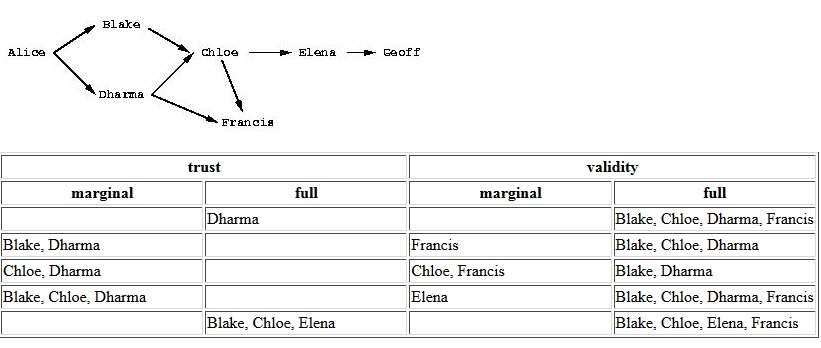
\includegraphics[scale=0.80]{graphics/trust_example.png}



\section{Couverture de test}

\begin{center}
    \begin{tabular}{|p{2.8cm}|p{4.2cm}|p{3cm}|p{5cm}|}
      \hline
      Id Exigence STB & Méthode de vérification & Procédure(s) utilisée(s) & Commentaire\\ \hline
      EF\_01 & La commande demandée a été exécutée avec les bons paramètres. & 1 & \\ \hline
      EF\_02 & Le chiffrement - déchiffrement - signature - vérification a été exécuté avec les bons paramètres. Un texte chiffré puis déchiffré doit être identique au texte de base. & 4,5,9 & \\ \hline
      EF\_03 & Chaque commande effectuée est affichée, avec retours et erreurs. & 6 & \\ \hline
      EF\_04 & Il doit y avoir au démarrage de l'application et à tout moment, la possibilité de changer de profil & 7 & \\ \hline
      EF\_05 & Tout changement de confiance est répercuté sur la toile de confiance. & 2 & \\ \hline
      EF\_06 & Pour une clé pgp donnée, on peut produire une autre clé ayant la même seconde pré-image. & 3 & \\ \hline
      EO\_01 & Effectuer tous les tests avec GnuPG 2.0.* & Toutes & \\ \hline
      EO\_02 & Effectuer tous les tests avec GnuPG 1.4.* & Toutes & \\ \hline
      EO\_03 & Effectuer tous les tests avec KDE 4.* et 5 & Toutes & \\ \hline
      EO\_04 & Effectuer tous les tests avec Gnome 3.* & Toutes & \\ \hline
      EO\_05 & Effectuer tous les tests sous Windows. & Toutes & \\ \hline
      EO\_06 & Vérifier que la toile de confiance s'affiche et représente correctement les niveaux de confiance. & 8 & \\ \hline
      EO\_07 & Ouvrir deux interfaces avec des profils différents sur la même session. & Toutes & \\ \hline
      EO\_08 & Vérifier que l'on peut s'authentifier en SSH via une clé signée par GPG. &  & \\ \hline
      EO\_09 & Rechercher des clés en local. &  & \\ \hline
      EQ\_01 & Chaque niveau de confiance est représenté par une couleur. & 8 & \\ \hline
      EQ\_03 & Effectuer tous les tests avec le paquet fourni. & Toutes & \\ \hline
  \end{tabular}  
\end{center}


\end{document}

